%% LyX 2.3.6.1 created this file.  For more info, see http://www.lyx.org/.
%% Do not edit unless you really know what you are doing.
\documentclass[english]{article}
\usepackage[T1]{fontenc}
\usepackage[latin9]{inputenc}
\usepackage{geometry}
\geometry{verbose,tmargin=2.5cm,bmargin=2.5cm,lmargin=2.5cm,rmargin=2.5cm}
\usepackage{calc}
\usepackage{graphicx}
\PassOptionsToPackage{normalem}{ulem}
\usepackage{ulem}

\makeatletter

%%%%%%%%%%%%%%%%%%%%%%%%%%%%%% LyX specific LaTeX commands.
%% Because html converters don't know tabularnewline
\providecommand{\tabularnewline}{\\}

\makeatother

\usepackage{babel}
\begin{document}
{[}SPLIT\_HERE{]}
\begin{enumerate}
\item \textbf{{[}JJC/PRELIM/9597/2018/P1/Q1{]} }

A web log, \texttt{WEBLOG.txt}, keeps track of the date and time the
server is being accessed, as well as the client that accessed it.
The client is identified by either the host name or internet address.
The format of \texttt{WEBLOG.txt} is as follows: 
\noindent \begin{center}
\texttt{<host name>|<DD/MMM/YYYY:HH:MM:SS> }
\par\end{center}

\noindent \begin{center}
\textbf{or }
\par\end{center}

\noindent \begin{center}
\texttt{<internet address>|<DD/MMM/YYYY:HH:MM:SS>} 
\par\end{center}

Below is a sample of \texttt{WEBLOG.txt}: 

\noindent\fbox{\begin{minipage}[t]{1\columnwidth - 2\fboxsep - 2\fboxrule}%
\texttt{199.72.81.55|01/Jul/2018:08:00:01 }

\texttt{jurongjc.moe.edu.sg|01/Jul/2018:09:08:06 }

\texttt{199.120.110.21|01/Jul/2018:11:30:09 }

\texttt{trioon.com|01/Jul/2018:11:45:58 }%
\end{minipage}}

A client address (host name or internet address) can appear in \texttt{WEBLOG.txt}
multiple times. Similarly, the date it accessed the server can be
duplicated because it can access the server more than once in a day. 

A summary report, \texttt{SUMMARYREPORT.txt}, is to be generated to
list the unique clients (hosts name/internet address) and their corresponding
dates. Below is a sample of \texttt{SUMMARYREPORT.txt}: 

\noindent\fbox{\begin{minipage}[t]{1\columnwidth - 2\fboxsep - 2\fboxrule}%
\texttt{199.72.81.55~~~~~~~ 01/Jul/2018,03/Jul/2018,04/Jul/2018 }

\texttt{jurongjc.moe.edu.sg 01/Jul/2018,02/Jul/2018,03/Jul/2018 }

\texttt{trioon.com ~~~~~~~~~01/Jul/2018,05/Jul/2018}%
\end{minipage}} 

\subsection*{Task 1.1 }

Write a procedure \texttt{readLog()} to read \texttt{WEBLOG.txt}.
Use suitable data structure(s), and prepare the log information to
create \texttt{SUMMARYREPORT.txt}.

\subsection*{Evidence 1: }

Your \texttt{readLog()} procedure code.\hfill{} {[}6{]}

\subsection*{Task 1.2 }

Write a procedure \texttt{processLog()} to generate \texttt{SUMMARYREPORT.txt}.

\subsection*{Evidence 2: }

Your \texttt{processLog()} procedure code.\hfill{} {[}4{]}

\subsection*{Evidence 3:}

Screenshot of \texttt{SUMMARYREPORT.txt} after running the program.\hfill{}
{[}1{]}

\subsection*{Task 1.3 }

Add code to your Task 1.2 program to display the highest number of
days the server was accessed by any client, and the corresponding
client(s). Below is a sample of screen output:

\noindent\fbox{\begin{minipage}[t]{1\columnwidth - 2\fboxsep - 2\fboxrule}%
\texttt{>\textcompwordmark >\textcompwordmark > Highest frequency
(days): 3 }

\texttt{>\textcompwordmark >\textcompwordmark > Accessed by: }

\texttt{>\textcompwordmark >\textcompwordmark > 199.72.81.55 }

\texttt{>\textcompwordmark >\textcompwordmark > jurongjc.moe.edu.sg }%
\end{minipage}}

\subsection*{Evidence 4:}

Your program code for \textbf{Task 1.3}.\hfill{} {[}4{]}

\subsection*{Evidence 5:}

Screenshot of the program output.\hfill{} {[}1{]}

{[}SPLIT\_HERE{]}
\item \textbf{{[}JJC/PRELIM/9597/2018/P1/Q2{]} }

The data file \texttt{COUNTRIES.txt} contains a list of country names. 

\subsection*{Task 2.1}

Write program code to store country names in \texttt{COUNTRIES.txt}
into an array, sort them in \textbf{descending} order using \textbf{insertion
sort} and output the sorted sequence. 

\subsection*{Evidence 6: }

Program code for Task 2.1 \hfill{} {[}7{]}

\subsection*{Evidence 7: }

Screenshot of the program output. \hfill{} {[}1{]}

\subsection*{Task 2.2 }

Write program code to store country names in \texttt{COUNTRIES.txt}
into an array, sort them in \textbf{ascending} order using \textbf{quicksort}
and output the sorted sequence. You may use the pseudocode in \texttt{QUICKSORT.txt}.
Do note the pseudocode is incomplete. You will have to fill in the
missing codes \texttt{A, B, C, D, E, F, G, H}. 

\subsection*{Evidence 8: }

Program code for \textbf{Task 2.2} \hfill{} {[}8{]}

\subsection*{Task 2.3 }

Write additional code to count and display the total number of comparisons
made in completing the quicksort process.

\subsection*{Evidence 9: }

Program code for \textbf{Task 2.3} to highlight the additional code
by using \textbf{bold} and \textbf{\emph{italics}}. \hfill{} {[}3{]}

\subsection*{Evidence 10:}

Screenshot of running Task 2.3.\hfill{} {[}1{]}

{[}SPLIT\_HERE{]}
\item \textbf{{[}JJC/PRELIM/9597/2018/P1/Q3{]} }

The class \texttt{Node} has the following properties and methods: 
\begin{center}
\begin{tabular}{|l|l|}
\hline 
\multicolumn{2}{|c|}{\texttt{Class: Node}}\tabularnewline
\hline 
\multicolumn{2}{|c|}{Attributes}\tabularnewline
\hline 
\texttt{\textbf{\hspace{0.01\columnwidth}}}\textbf{Identifier} & \texttt{\textbf{\hspace{0.05\columnwidth}}}\textbf{Description}\tabularnewline
\hline 
\texttt{data : String} & Data stored at the node.\tabularnewline
\hline 
\texttt{left : INTEGER} & Points to the left child of the node. Implement 0 as NULL value. \tabularnewline
\hline 
\texttt{right : INTEGER } & Points to the right child of the node. Implement 0 as NULL value.\tabularnewline
\hline 
\multicolumn{2}{|l|}{Methods}\tabularnewline
\hline 
\texttt{Constructor()} & Initialises an instance of \texttt{Node}. \tabularnewline
\hline 
\texttt{set\_data(data : String)} & Modifier method for \texttt{data}.\tabularnewline
\hline 
\texttt{get\_data() : String} & Accessor method for \texttt{data}. \tabularnewline
\hline 
\texttt{set\_left(index : INTEGER)} & Modifier method for \texttt{left}.\tabularnewline
\hline 
\texttt{get\_left() : INTEGER} & Accessor method for \texttt{left}\tabularnewline
\hline 
\texttt{set\_right(index : INTEGER)} & Modifier method for \texttt{right}.\tabularnewline
\hline 
\texttt{get\_right() : INTEGER} & Accessor method for \texttt{right}.\tabularnewline
\hline 
\end{tabular}
\par\end{center}

\subsection*{Task 3.1 }

Write program code for the class \texttt{Node}. 

\subsection*{Evidence 11:}

Program code for Task 3.1.\hfill{} {[}4{]}

The class \texttt{BinarySearchTree} has the following properties and
methods: 
\begin{itemize}
\item Properties 
\begin{itemize}
\item \texttt{root : INTEGER} Points to the root of binary search tree.
Implement 0 as NULL value. 
\item \texttt{nodes : ARRAY{[}31{]} OF Node} The array index starts at 1
and the dataset (i.e.: binary search tree) has a maximum of 31 Node
objects. 
\item \texttt{nextFree : INTEGER} Index for the next unused node. 
\end{itemize}
\item Methods 
\begin{itemize}
\item \texttt{Constructor()} Initialises the \texttt{root}, \texttt{nextFree}
and nodes of \texttt{BinarySearchTree}. 
\item \texttt{addNode(data : String)} Inserts new node into binary search
tree. 

The \texttt{data} of each parent node is larger than the \texttt{data}
of its left child. 
\item \texttt{set\_root(index : INTEGER)} Modifier method for root. 
\item \texttt{get\_root() : INTEGER} Accessor method for root. 
\item \texttt{searchNode(item : String) : BOOLEAN} Searches if \texttt{item}
is stored in one of the nodes of the binary search tree. 

Returns \texttt{TRUE} if found and \texttt{FALSE} otherwise. 
\item \texttt{inOrderTraversal(root : INTEGER)} Displays the \texttt{data}
of each \texttt{node} stored in the binary search tree when traversed
using an inorder algorithm. 

For example: 
\begin{center}
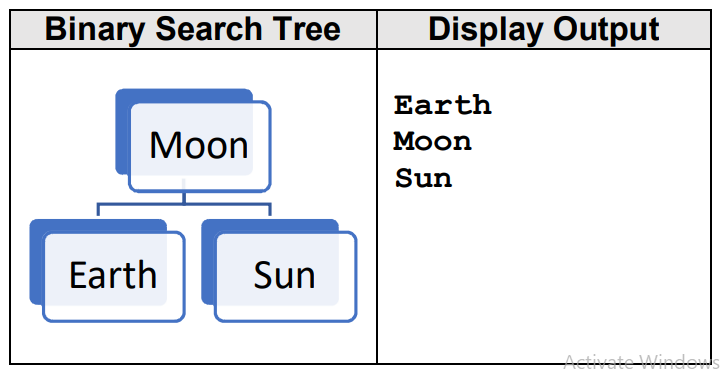
\includegraphics[width=0.5\paperwidth]{C:/Users/Admin/Desktop/Github/question_bank/LyX/static/img/9597-JJC-2018-P1-Q3-1}
\par\end{center}
\item \texttt{balance() : BinarySearchTree} Traverses the binary search
tree to return a new balanced binary search tree. A \textbf{recursive}
algorithm is required. 
\end{itemize}
\end{itemize}

\subsection*{Task 3.2 }

Write program code for the class \texttt{BinarySearchTree}. You may
assume space will not be reused should any node be deleted and the
binary search tree will not be full. 

\subsection*{Evidence 12: }

Program code for Task 3.2. \hfill{}{[}18{]}

The class \texttt{HashTable} has the following properties and methods:

\subsection*{Task 3.3}

Write program code for the class HashTable.
\begin{itemize}
\item properties
\begin{itemize}
\item \texttt{size : INTEGER} Number of items in the hash table array.
\item \texttt{hashTableArray : ARRAY{[}size{]} OF BinarySearchTree} An array
storing \texttt{BinarySearchTree} objects from indices 0 to size -1. 
\end{itemize}
\item methods
\begin{itemize}
\item \texttt{Constructor(size : INTEGER)} Initialises the \texttt{size}
and \texttt{hashTableArray} of \texttt{HashTable}. 
\item \texttt{hash(key : String) : INTEGER} A hashing function that calculates
the address of the hash table. 

Takes \texttt{key}, a String, as an argument. The last six characters
in \texttt{key} are digits.

\textbf{Sums each of the first three digits}, divides the total by
\texttt{size} and returns the remainder. 

For example, where \texttt{size} is 5: 

\noindent\begin{minipage}[t]{1\columnwidth}%
\texttt{hash(\textquotedblleft 111JalanTenteram}\texttt{\textbf{322111}}\texttt{\textquotedblright )}

\texttt{>\textcompwordmark >\textcompwordmark > 2 }

\texttt{hash(\textquotedblleft 23PasirRisAve}\texttt{\textbf{4520021}}\texttt{\textquotedblright )}

\texttt{>\textcompwordmark >\textcompwordmark > 2 }%
\end{minipage}
\end{itemize}
\end{itemize}

\subsection*{Evidence 13: }

Program code for Task 3.3.\hfill{} {[}4{]}

ACE OF CODERS PTE LTD would like to conduct a lucky draw. Each customer
is entitled to submit one entry. All customer data entered is stored
in the text file \texttt{CUSTOMERDATA.txt}. The format of the text
file is as follows: 
\noindent \begin{center}
\texttt{<CUSTOMER NAME> <CONTACT NUMBER>|<ADDRESS> }
\par\end{center}

Below is a sample of \texttt{CUSTOMERDATA.txt}: 

\noindent\fbox{\begin{minipage}[t]{1\columnwidth - 2\fboxsep - 2\fboxrule}%
\texttt{Felicia Lee Si Ying 98635610}\texttt{\textbf{|}}\texttt{19JalanTenteram322019 }

\texttt{Yap Chee How 67767515}\texttt{\textbf{|}}\texttt{23TohTuckDrive608023 }

\texttt{Christy Lopez 92233123}\texttt{\textbf{|}}\texttt{507WestCoastRoad120507 }%
\end{minipage}}

There will be five lucky draw winners. The company has identified
five regions in Singapore and would like to pick one winner from each
region. The hashing function from Task 3.3 \uline{will categorise
an address in one of the five regions}. 

\subsection*{Task 3.4 }

Using the classes programmed previously, code a main program that
repeatedly: 
\begin{itemize}
\item displays the following menu:

\noindent\fbox{\begin{minipage}[t]{1\columnwidth - 2\fboxsep - 2\fboxrule}%
\texttt{1. Prepare hash table}

\texttt{2. Generate winners}

\texttt{3. Search for entry }%
\end{minipage}}
\item calls an appropriate procedure depending on the user\textquoteright s
choice
\end{itemize}
When implementing the choices, take note of the following: 
\begin{enumerate}
\item[1.] \textbf{ Prepare hash table} 

User inputs suitable size of hash table to be initialised.

Reads customer data from \texttt{CUSTOMERDATA.txt}. 

Uses address as key and customer name, contact number as value.

Stores the customer names, contact numbers into the hash table. 
\item[2.] \textbf{ Generate winners} 

Randomly select one winner from each binary search tree in the hash
table.

Display their names and contact numbers. 
\item[3.]  \textbf{Search for entry} 

Staff of the company may not enter the lucky draw. 

Displays whether the staff name and contact number entered by user
exists in the hash table. 
\end{enumerate}

\subsection*{Evidence 14: }

Program code for Task 3.4. \hfill{}{[}10{]}

\subsection*{Task 3.5}

Run your program. Complete choice 1 before searching the following. 

\noindent\begin{minipage}[t]{1\columnwidth}%
\texttt{>\textcompwordmark >\textcompwordmark > Sandra Chelvan 92233123 }

\texttt{>\textcompwordmark >\textcompwordmark > Haz Awang 87767888 }

\texttt{>\textcompwordmark >\textcompwordmark > Seah Hon Hui 91144000 }%
\end{minipage}

\subsection*{Evidence 15:}

Screenshot of running Task 3.5. \hfill{}{[}2{]}

{[}SPLIT\_HERE{]}
\item \textbf{{[}JJC/PRELIM/9597/2018/P1/Q4{]} }

Rock Paper Scissors is a well-known hand game played between two players,
whom we shall call P1 and P2. For each round, each player simultaneously
forms one of three signs with an outstretched hand. Rock (represented
by \textquotedbl 0\textquotedbl ), scissors (represented by \textquotedbl 2\textquotedbl )
and paper (represented by \textquotedbl 5\textquotedbl ).

Program \texttt{get\_round\_winner(p1\_hand, p2\_hand)} that decides
who wins from the hand signs of P1 and P2. If P1 wins, the function
returns 1. If P2 wins, the function returns 2. If the game is a draw,
the function returns 0.

Sample Execution:

\noindent\begin{minipage}[t]{1\columnwidth}%
\texttt{get\_round\_winner (\textquotedbl 2\textquotedbl , \textquotedbl 5\textquotedbl )
\# scissors vs paper - P1 wins}

\texttt{>\textcompwordmark >\textcompwordmark > 1}

\texttt{get\_round\_winner (\textquotedbl 2\textquotedbl , \textquotedbl 0\textquotedbl )
\# scissors vs rock - P2 wins }

\texttt{>\textcompwordmark >\textcompwordmark > 2 }

\texttt{get\_round\_winner (\textquotedbl 2\textquotedbl , \textquotedbl 2\textquotedbl )
\# scissors vs scissors - Draw}

\texttt{>\textcompwordmark >\textcompwordmark > 0}%
\end{minipage}

\subsection*{Task 4.1 }

Write program code for the function\texttt{ get\_round\_winner}.

\subsection*{Evidence 16: }

Program code for \textbf{Task 4.1}.\hfill{} {[}4{]}

P1 and P2 played a game of Rock Paper Scissors over a few rounds.
The winner is the player who wins more rounds than he losses. A draw
occurs if there is no winner. The hand signs of each player for the
game are represented as a string of \textquotedbl 0\textquotedbl ,
\textquotedbl 2\textquotedbl{} and \textquotedbl 5\textquotedbl .
For example, \textquotedbl 205\textquotedbl{} represents playing
scissors in the first round, rock in the second, and paper in the
third. 

Program \texttt{get\_game\_winner(p1\_hands, p2\_hands)} that decides
who wins the game from a sequence of hand signs from P1 and P2. If
P1 wins, return 1, if P2 wins, return 2, if the game is a draw, return
0. You must use \texttt{get\_round\_winner}. You may assume that \texttt{p1\_hands}
and \texttt{p2\_hands} are strings of the same length containing only
\textquotedbl 0\textquotedbl , \textquotedbl 2\textquotedbl{} and
\textquotedbl 5\textquotedbl . 

Sample Execution:

\noindent\begin{minipage}[t]{1\columnwidth}%
\texttt{get\_game\_winner (\textquotedbl\textquotedbl , \textquotedbl\textquotedbl )
\#no hand played, game ends in a draw}

\texttt{>\textcompwordmark >\textcompwordmark > 0}

\texttt{get\_game\_winner (\textquotedbl 205\textquotedbl , \textquotedbl 520\textquotedbl )
\#P1 wins all 3 rounds, P1 wins }

\texttt{>\textcompwordmark >\textcompwordmark > 1 }

\texttt{get\_game\_winner (\textquotedbl 22222\textquotedbl , \textquotedbl 50505\textquotedbl )
\#P1 wins}

\texttt{>\textcompwordmark >\textcompwordmark > 1 }

\texttt{get\_game\_winner (\textquotedbl 2050\textquotedbl , \textquotedbl 0255\textquotedbl )
\#P2 wins }

\texttt{>\textcompwordmark >\textcompwordmark > 2 }

\texttt{get\_game\_winner (\textquotedbl 52025\textquotedbl , \textquotedbl 52025\textquotedbl )
\#Draw }

\texttt{>\textcompwordmark >\textcompwordmark > 0 }%
\end{minipage}

\subsection*{Task 4.2 }

Write program code for the function \texttt{get\_game\_winner}. 

\subsection*{Evidence 17: }

Program code for Task 4.2. \hfill{}{[}6{]}

P1 and P2 would like a more interesting interface where rows and columns
display the game played. \textbf{Each game has four rounds} and the
\textbf{overall result} (\textquotedblleft P1 wins\textquotedblright ,
\textquotedblleft P2 wins\textquotedblright{} or \textquotedblleft Draw\textquotedblright )
\textbf{will be displayed when the game is over}. 

Here is a sample screenshot of the first turns taken by player. 

\noindent\begin{minipage}[t]{1\columnwidth}%
\texttt{Round ~~~~~~~P1 ~~~~~~~P2 ~~~~~~~Round
Winner}

\texttt{1 ~~~~~~~~~~~- ~~~~~~~~- ~~~~~~~~- }

\texttt{2 ~~~~~~~~~~~- ~~~~~~~~- ~~~~~~~~- }

\texttt{3 ~~~~~~~~~~~- ~~~~~~~~- ~~~~~~~~- }

\texttt{4 ~~~~~~~~~~~- ~~~~~~~~- ~~~~~~~~- }

\texttt{Player's 1 turn.}

\texttt{Enter Rock (0), Paper (5) or Scissors (2): 2}

\texttt{Round ~~~~~~~P1 ~~~~~~~P2 ~~~~~~~Round
Winner}

\texttt{1 ~~~~~~~~~~~S ~~~~~~~~- ~~~~~~~~- }

\texttt{2 ~~~~~~~~~~~- ~~~~~~~~- ~~~~~~~~- }

\texttt{3 ~~~~~~~~~~~- ~~~~~~~~- ~~~~~~~~- }

\texttt{4 ~~~~~~~~~~~- ~~~~~~~~- ~~~~~~~~- }

\texttt{Player's 2 turn.}

\texttt{Enter Rock (0), Paper (5) or Scissors (2): 0}

\texttt{Round ~~~~~~~P1 ~~~~~~~P2 ~~~~~~~Round
Winner}

\texttt{1 ~~~~~~~~~~~S ~~~~~~~~R ~~~~~~~~P2 }

\texttt{2 ~~~~~~~~~~~- ~~~~~~~~- ~~~~~~~~- }

\texttt{3 ~~~~~~~~~~~- ~~~~~~~~- ~~~~~~~~- }

\texttt{4 ~~~~~~~~~~~- ~~~~~~~~- ~~~~~~~~- }%
\end{minipage}

\subsection*{Task 4.3 }

Write program code for the game described. Implement using \textbf{modularity}
and\textbf{ 2D array}. Include function \texttt{validate()} to ensure
the player chooses \texttt{0}, \texttt{2} or \texttt{5}. Prompt the
player to re-enter if input is invalid. 

\subsection*{Evidence 18: }

Program code for Task 4.3.\hfill{} {[}10{]}

\subsection*{Evidence 19: }

Design four appropriate test cases for the program. Present them in
a table format. \hfill{}{[}4{]}

\subsection*{Evidence 20: }

Run your program and produce screenshots for a game which ends in
a draw and another game which P1 wins.\hfill{} {[}2{]}

{[}SPLIT\_HERE{]}
\item \textbf{{[}JJC/PRELIM/9597/2018/P2/Q1{]} }

J \& J Dental Care has a team of freelance dentists. As there are
two dental treatment rooms in the clinic, only two dentists may be
on duty each day. The clinic manager finalises the monthly duty roster
a week before the new month commences. Every patient has to either
call or visit the clinic to book an appointment. The receptionist
handling the booking will require the following details: 
\begin{itemize}
\item patient name 
\item postal code 
\item dentist requested (optional)
\item date requested 
\end{itemize}
The receptionist checks the hard copy files to ensure that the patient
is registered with the clinic and views the availability in the appointments
book. After the dentist, date and time have been finalised, the patient\textquoteright s
appointment will be recorded in the appointments book.

At the beginning of each day, the receptionist types an appointment
list for each of the dentists working that day. The list contains
patients\textquoteright{} names and their respective timings. 

When patients arrive at the clinic for their appointments, they announce
their names to the receptionist and the receptionist will enter the
treatment rooms to inform the dentists. 

The clinic has decided to replace this manual system with a computerised
system. 

A system developer is employed to carry out the project. The first
task assigned to the system developer is to write a project proposal.
\begin{enumerate}
\item One section of the project proposal is the Problem Statement which
lists the problems in the current system. Write the Problem Statement.
\hfill{}{[}4{]}
\item Explain why the problem must be defined accurately. \hfill{}{[}2{]}
\item Describe and justify three methods which can be used to determine
the requirements for the computerised system.\hfill{} {[}6{]}
\item As a result of the analysis carried out, a diagram is used to show
entities and data flow of the \uline{appointment booking process
only}. Draw a suitable diagram.\hfill{} {[}6{]}
\end{enumerate}
The system developer has drawn up an initial plan of the work involved: 
\noindent \begin{center}
\begin{tabular}{|c|l|c|}
\hline 
\textbf{Stage} & \textbf{Activity} & \textbf{Weeks}\tabularnewline
\hline 
A & Produce design & 5\tabularnewline
\hline 
B & Identify requirements & 3\tabularnewline
\hline 
C & Implement code & 9\tabularnewline
\hline 
D & Perform black box testing & 2\tabularnewline
\hline 
E & Perform acceptance testing & 3\tabularnewline
\hline 
F & Prepare documentation & 6\tabularnewline
\hline 
\end{tabular} 
\par\end{center}

From the work breakdown, a Program Evaluation Review Technique (PERT)
chart is constructed. 
\begin{center}
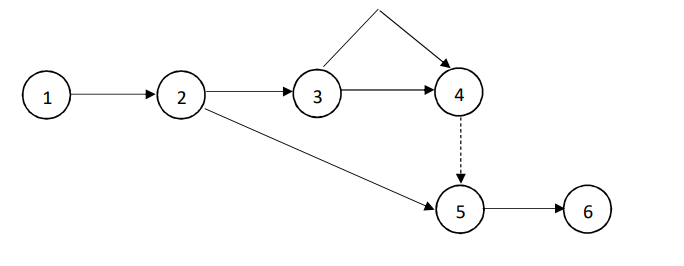
\includegraphics[width=0.5\paperwidth]{C:/Users/Admin/Desktop/Github/question_bank/LyX/static/img/9597-JJC-2018-P2-Q1-1}
\par\end{center}
\begin{enumerate}
\item[(e)]  Complete the PERT chart by adding the stages and their respective
durations in the correct sequence.\hfill{} {[}4{]}
\item[(f)]  State the critical path.\hfill{} {[}1{]}
\item[(g)]  State the minimum time in which the project could be completed.\hfill{}
{[}1{]}
\item[(h)]  The first activity commences at Week 0. For activity D: 
\begin{itemize}
\item state the earliest start time. 
\item state the latest finish time.\hfill{}{[}2{]}
\end{itemize}
\item[(i)]  Two stages start and end at the same nodes. 
\begin{itemize}
\item Re-draw the PERT chart by using an additional dummy stage separating
them. 
\item Explain the purpose of the dummy stage. \hfill{} {[}2{]}
\end{itemize}
\item[(j)]  List two types of documentation produced for this project. \hfill{}{[}2{]}
\end{enumerate}
The computerised system will use a database. In the updated system
the dentists will be given a hand-held device, that is networked,
to use in their rooms for accessing the patient records. 
\begin{enumerate}
\item[(k)]  Describe two other uses for the hand-held device. \hfill{} {[}2{]}
\item[(l)]  Describe a possible ethical concern raised by this new system. \hfill{}{[}2{]}
\item[(m)] An alternative solution for this project is to use cloud computing.
Describe how each of the three types of cloud computing services may
be used for the new project. \hfill{} {[}6{]}
\end{enumerate}
{[}SPLIT\_HERE{]}
\item \textbf{{[}JJC/PRELIM/9597/2018/P2/Q2{]} }

The following are examples of hard copy documents managed by the receptionist
at J \& J Dental Care. 

\noindent\fbox{\begin{minipage}[t]{1\columnwidth - 2\fboxsep - 2\fboxrule}%
Patient name: Mark Lee Xiao Ming 

Patient address: 17 Toh Tuck Road, Singapore 596017 

Contact number: 67767515

Allergies: None%
\end{minipage}}
\noindent \begin{center}
Figure 1: Patient Record
\par\end{center}

\begin{center}
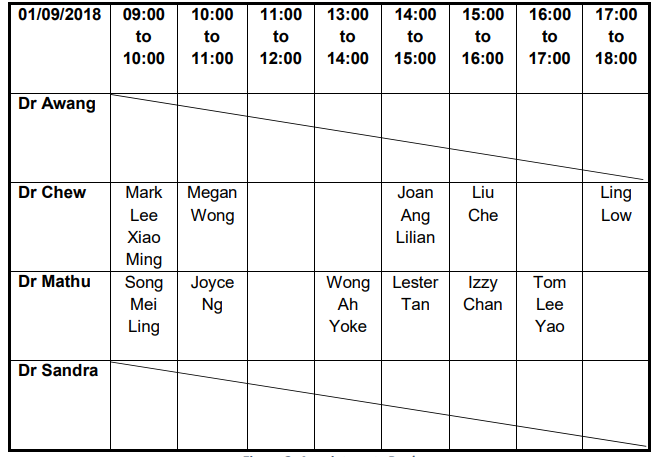
\includegraphics[width=0.5\paperwidth]{C:/Users/Admin/Desktop/Github/question_bank/LyX/static/img/9597-JJC-2018-P2-Q2-1}
\par\end{center}

\noindent \begin{center}
Figure 2: Appointments Book 
\par\end{center}

\noindent\fbox{\begin{minipage}[t]{1\columnwidth - 2\fboxsep - 2\fboxrule}%
Date: 01/09/2018 

Dentist name: Dr Mathu 

09:00: Song Mei Ling 

10:00: Joyce Ng

\dots{} \dots{}

\bigskip{}
%
\end{minipage}}
\noindent \begin{center}
Figure 3: Appointment List
\par\end{center}

\noindent\fbox{\begin{minipage}[t]{1\columnwidth - 2\fboxsep - 2\fboxrule}%
Dentist name: Dr Mathu 

Dentist address: 6 West Coast Drive, Singapore 120006 

Contact number: 98833567%
\end{minipage}}
\noindent \begin{center}
Figure 4: Dentist Record
\par\end{center}
\begin{enumerate}
\item Explain why the patient name and postal code are needed when the receptionist
handles an appointment booking for a patient. \hfill{}{[}2{]}
\item Explain, using two examples, how such a system may compromise data
integrity. \hfill{}{[}4{]}
\item Describe, using an example, how such a system has data redundancy.
\hfill{}{[}2{]}
\item Each patient may book a maximum of one appointment per day. A fully
normalised database solution to this problem is designed. Draw an
E-R diagram that shows these tables and the relationships between
them. \hfill{}{[}4{]}
\item Hence, write the table descriptions. You may introduce additional
attribute(s). Underline the primary keys.\hfill{} {[}3{]}
\item State three fields that require data validation. Suggest a suitable
type of check for each field. \hfill{}{[}3{]}
\end{enumerate}
{[}SPLIT\_HERE{]}
\item \textbf{{[}JJC/PRELIM/9597/2018/P2/Q3{]} }

The following is a byte stored in a file which contains binary code: 
\noindent \begin{center}
\texttt{01101001}
\par\end{center}
\begin{enumerate}
\item What is the corresponding denary number? \hfill{}{[}1{]}
\item What is the corresponding octal number?\hfill{} {[}1{]}
\item An operating system provides a user interface to a computer system.
List two types of interface that an operating system provides and
state an advantage for each. \hfill{}{[}4{]}
\item Many modern operating systems support Unicode. 
\begin{itemize}
\item What is Unicode? 
\item What are two advantages of Unicode over ASCII? \hfill{}{[}3{]}
\end{itemize}
\end{enumerate}
{[}SPLIT\_HERE{]}
\item \textbf{{[}JJC/PRELIM/9597/2018/P2/Q4{]} }

An object-oriented program is being written to store details about
clients at a real estate agency. 

Clients can be either sellers or prospective buyers. A class \texttt{Client}
has been created and two subclasses, \texttt{Seller} and \texttt{Buyer}
are to be developed. A \texttt{Location} class has been created to
store details about an address (e.g. postal code, street name and
district). 

The \texttt{Client} class has data fields \texttt{Name}, \texttt{Address}
and \texttt{DOB}. Part of the class definition for \texttt{Client}
class is: 

\noindent\begin{minipage}[t]{1\columnwidth}%
\texttt{Client = Class}

\texttt{\qquad{}// Private }

\texttt{\qquad{}Name: String}

\texttt{\qquad{}Address: Location }

\texttt{\qquad{}DOB: Date}

\bigskip{}

\texttt{\qquad{}// Public }

\texttt{\qquad{}Constructor() }

\texttt{\qquad{}Function GetName(): String }

\texttt{\qquad{}Function GetDOB(): Date Function}

\texttt{\qquad{}GetAddress(): Location }

\texttt{\qquad{}Procedure SetDetails(String, Location, Date) }%
\end{minipage}

A \texttt{Buyer} has the following additional data fields: 
\begin{itemize}
\item \texttt{NoOfBedroomsRequired}: stores the minimum number of bedrooms
that the buyer requires in the property they purchase.
\item \texttt{ParkingSpace}: stores a value indicating if the buyer requires
parking or not. 
\item \texttt{AreaDesired}: the district the buyer is looking to purchase
a property in. For example, Jurong is in district 22 while Orchard
is in district 9. 
\end{itemize}
\begin{enumerate}
\item Write the class definition for \texttt{Buyer}. \hfill{}{[}4{]}
\item Hence, illustrate the diagram which exhibits the relationships between
all classes as well as inheritance and encapsulation. \hfill{}{[}6{]}
\item Explain why encapsulation is an important feature of object-oriented
programming. \hfill{}{[}2{]}
\end{enumerate}
{[}SPLIT\_HERE{]}
\item \textbf{{[}JJC/PRELIM/9597/2018/P2/Q5{]} }

The following shows a message being encrypted using a Caesar cipher.
\begin{center}
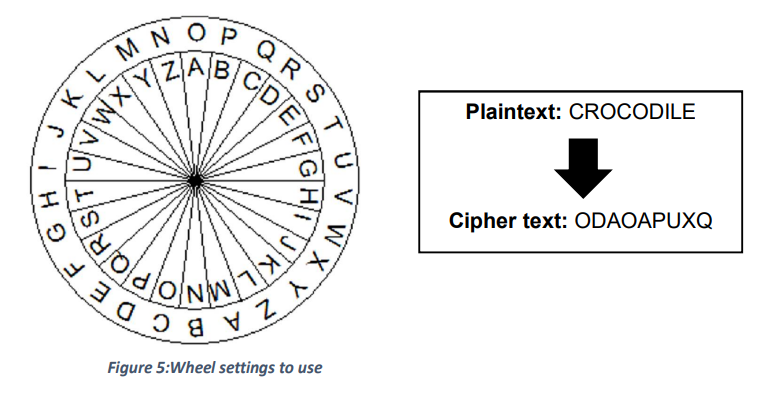
\includegraphics[width=0.5\paperwidth]{C:/Users/Admin/Desktop/Github/question_bank/LyX/static/img/9597-JJC-2018-P2-Q5-1}
\par\end{center}
\begin{enumerate}
\item Decrypt the cipher text \textquotedbl\textbf{QXQBTMZF}\textquotedbl{}
using the Caesar cipher with the settings shown in Figure 5. \hfill{}{[}1{]}
\end{enumerate}
In modern terminology, a Vernam cipher is a symmetrical stream cipher
in which the plaintext is combined with a random or pseudorandom stream
of data (the \textquotedbl keystream\textquotedbl ) of the same
length, to generate the cipher text, using the Boolean \textquotedbl exclusive
or\textquotedbl{} (XOR) function. 
\noindent \begin{center}
\begin{tabular}{|c|c|c|}
\hline 
A & B & A \textbf{XOR} B\tabularnewline
\hline 
0 & 0 & 0\tabularnewline
\hline 
0 & 1 & 1\tabularnewline
\hline 
1 & 0 & 1\tabularnewline
\hline 
1 & 1 & 0\tabularnewline
\hline 
\end{tabular}
\par\end{center}

Using the Vernam cipher method, the plaintext \textquotedbl RUN\textquotedbl{}
is to be encrypted. \textquotedbl RUN\textquotedbl{} will be encoded
using 8-bit ASCII, according to the following ASCII table. 
\noindent \begin{center}
\begin{tabular}{|c|c|c|c|c|c|}
\hline 
Letter & ASCII Code & Letter & ASCII Code & Letter & ASCII Code\tabularnewline
\hline 
A & 01000001 & J & 01001010 & S & 01010011\tabularnewline
\hline 
B & 01000010 & K & 01001011 & T & 01010100\tabularnewline
\hline 
C & 01000011 & L & 01001100 & U & 01010101\tabularnewline
\hline 
D & 01000100 & M & 01001101 & V & 01010110\tabularnewline
\hline 
E & 01000101 & N & 01001110 & W & 01010111\tabularnewline
\hline 
F & 01000110 & O & 01001111 & X & 01011000\tabularnewline
\hline 
G & 01000111 & P & 01010000 & Y & 01011001\tabularnewline
\hline 
H & 01001000 & Q & 01010001 & Z & 01011010\tabularnewline
\hline 
I & 01001001 & R & 01010010 & \multicolumn{1}{c}{} & \multicolumn{1}{c}{}\tabularnewline
\cline{1-4} \cline{2-4} \cline{3-4} \cline{4-4} 
\end{tabular}
\par\end{center}
\begin{enumerate}
\item[(b)]  The key \texttt{10111001} \texttt{01001101} \texttt{01000001} will
be used to perform the encryption. Perform this encryption. Show your
working to derive the cipher text from the plain text. \hfill{}{[}3{]}
\item[(c)]  Both the Caesar and Vernam ciphers are symmetric ciphers. Explain
the difference between a symmetric and an asymmetric cipher system.
\hfill{}{[}1{]}
\end{enumerate}
The following diagram shows the physical topology of a typical home
Local Area Network (LAN) and its connection to the Internet. The LAN
uses the IPv4 protocol. 

Device A is a Wireless Access Point. A range of devices, including
laptop computers and mobile phones connect to the network through
the Wireless Access Point.

Device B is a Network Attached Storage device which is a server used
to store files that can be accessed by other devices connected to
the network. 
\begin{center}
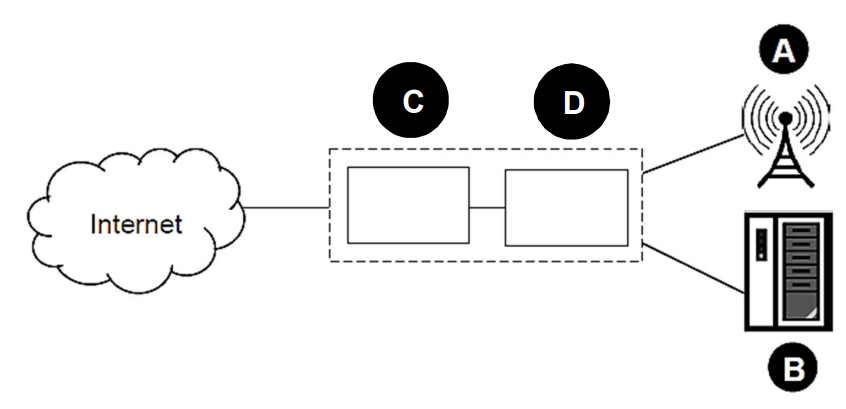
\includegraphics[width=0.5\paperwidth]{C:/Users/Admin/Desktop/Github/question_bank/LyX/static/img/9597-JJC-2018-P2-Q5-2}
\par\end{center}
\begin{enumerate}
\item[(d)]  Identify the two networking devices (C and D). \hfill{}{[}2{]}
\item[(e)]  The devices that are used within the home have private IP addresses.
The Combined Device has both a private IP address and a public IP
address. Explain the differences between private and public IP addresses,
and why the Combined Device has both.\hfill{} {[}3{]}
\item[(f)]  Describe two methods for ensuring the security of access to the
files in Device B. \hfill{}{[}4{]}
\end{enumerate}
{[}SPLIT\_HERE{]}
\item \textbf{{[}JJC/PRELIM/9597/2018/P2/Q6{]} }

The following pseudo-code contains an algorithm called \texttt{Merge}
that is called by the \texttt{MergeSort} algorithm. 

\noindent %
\noindent\begin{minipage}[t]{1\columnwidth}%
\texttt{FUNCTION MergeSort(L, S, E)}

\texttt{\qquad{}IF S < E THEN }

\texttt{\qquad{}\qquad{}M <- (S + E) DIV 2 }

\texttt{\qquad{}\qquad{}L1 <- MergeSort(L, S, M) }

\texttt{\qquad{}\qquad{}L2 <- MergeSort(L, M + 1, E) }

\texttt{\qquad{}\qquad{}RETURN Merge(L1, L2)}

\texttt{\qquad{}ELSE }

\texttt{\qquad{}\qquad{}RETURN Append({[}{]}, L{[}S{]}) }

\texttt{\qquad{}ENDIF}

\texttt{ENDFUNCTION}

\bigskip{}

\texttt{FUNCTION Merge(L1, L2) }

\texttt{\qquad{}L3 <- {[}{]} }

\texttt{\qquad{}WHILE Len(L1) > 0 AND LEN(L2) > 0}

\texttt{\qquad{}\qquad{}IF L1{[}1{]} < L2{[}1{]} THEN }

\texttt{\qquad{}\qquad{}\qquad{}L3 <- Append(L2{[}1{]}, L3) }

\texttt{\qquad{}\qquad{}\qquad{}L2 <- RemoveFirstItem(L2) }

\texttt{\qquad{}\qquad{}ELSE }

\texttt{\qquad{}\qquad{}\qquad{}L3 <- Append(L1{[}1{]}, L3) }

\texttt{\qquad{}\qquad{}\qquad{}L1 <- RemoveFirstItem(L1) }

\texttt{\qquad{}\qquad{}ENDIF}

\texttt{\qquad{}ENDWHILE}

\texttt{\qquad{}WHILE Len(L1) > 0}

\texttt{\qquad{}\qquad{}L3 <- Append(L1{[}1{]}, L3) }

\texttt{\qquad{}\qquad{}L1 <- RemoveFirstItem(L1) }

\texttt{\qquad{}ENDWHILE }

\texttt{\qquad{}WHILE Len(L2) > 0 }

\texttt{\qquad{}\qquad{}L3 <- Append(L2{[}1{]}, L3)}

\texttt{\qquad{}\qquad{}L2 <- RemoveFirstItem(L2) }

\texttt{\qquad{}ENDWHILE }

\texttt{\qquad{}RETURN L3}

\texttt{ENDFUNCTION} %
\end{minipage}

The \texttt{RemoveFirstItem} function takes a list and returns a list
that contains all the items in the original list except the first
one. For example, if \texttt{Names} is the list {[}\textquotedbl\texttt{Gemma}\textquotedbl ,
\textquotedbl\texttt{Richard}\textquotedbl , \textquotedbl\texttt{Georgina}\textquotedbl ,
\textquotedbl\texttt{Margaret}\textquotedbl{]} then the function
call \texttt{RemoveFirstItem(Names)} will return the list {[}\textquotedbl\texttt{Richard}\textquotedbl ,
\textquotedbl\texttt{Georgina}\textquotedbl , \textquotedbl\texttt{Margaret}\textquotedbl{]}. 

The \texttt{Len} function takes a list and returns the number of items
that are in the list. For example, if \texttt{Names} is the list {[}\textquotedbl\texttt{Gemma}\textquotedbl ,
\textquotedbl\texttt{Richard}\textquotedbl , \textquotedbl\texttt{Georgina}\textquotedbl ,
\textquotedbl\texttt{Margaret}\textquotedbl{]} then the function
call \texttt{Len(Names)} will return the value of 4. 

The \texttt{Append} function takes an item and a list and returns
a list that has all the items from the original list followed by the
item. For example, if \texttt{Names} is the list {[}\textquotedbl\texttt{Gemma}\textquotedbl ,
\textquotedbl\texttt{Richard}\textquotedbl , \textquotedbl\texttt{Georgina}\textquotedbl ,
\textquotedbl\texttt{Margaret}\textquotedbl{]} then the function
call\texttt{ Append(\textquotedbl Matt\textquotedbl , Names)} will
return the list {[}\textquotedbl\texttt{Gemma}\textquotedbl , \textquotedbl\texttt{Richard}\textquotedbl ,
\textquotedbl\texttt{Georgina}\textquotedbl , \textquotedbl\texttt{Margaret}\textquotedbl ,
\textquotedbl\texttt{Matt}\textquotedbl{]}.

The first item in the list has an index of 1. 
\begin{enumerate}
\item What is meant by a recursive subroutine? \hfill{}{[}1{]}
\item What is the base case for the subroutine \texttt{MergeSort}? \hfill{}
{[}1{]}
\item Complete the following table to show the result of tracing \texttt{MergeSort}
with the function call \texttt{MergeSort(ListToSort, 1, 5)}. \hfill{}{[}4{]}
\end{enumerate}
\texttt{ListToSort} is the list \texttt{{[}6, 3, 4, 8, 5{]}}. The
first six rows and the call number column have been completed for
you. 
\noindent \begin{center}
\begin{tabular}{|c|c|c|c|c|}
\hline 
\textbf{Call number} & \textbf{S} & \textbf{E} & \textbf{M} & \textbf{List returned}\tabularnewline
\hline 
1 & 1 & 5 & 3 & \tabularnewline
\hline 
2 & 1 & 3 & 2 & \tabularnewline
\hline 
3 & 1 & 2 & 1 & \tabularnewline
\hline 
4 & 1 & 1 &  & {[}6{]}\tabularnewline
\hline 
3 & 1 & 2 & 1 & \tabularnewline
\hline 
5 & 2 & 2 &  & {[}3{]}\tabularnewline
\hline 
3 &  &  &  & \tabularnewline
\hline 
2 &  &  &  & \tabularnewline
\hline 
6 &  &  &  & \tabularnewline
\hline 
2 &  &  &  & \tabularnewline
\hline 
1 &  &  &  & \tabularnewline
\hline 
7 &  &  &  & \tabularnewline
\hline 
8 &  &  &  & \tabularnewline
\hline 
7 &  &  &  & \tabularnewline
\hline 
9 &  &  &  & \tabularnewline
\hline 
7 &  &  &  & \tabularnewline
\hline 
1 &  &  &  & \tabularnewline
\hline 
\end{tabular}
\par\end{center}
\begin{enumerate}
\item[(d) ] What is the time complexity for the MergeSort algorithm? \hfill{}
{[}1{]}
\end{enumerate}
{[}SPLIT\_HERE{]}
\end{enumerate}

\end{document}
